\documentclass{article}
\usepackage[utf8]{inputenc}
\usepackage{fancyhdr}
\usepackage[margin=1.0in]{geometry}
\usepackage{amsmath}
\usepackage{changepage}
\usepackage{graphicx}
\usepackage[inline]{enumitem}
\usepackage{enumitem}
\pagestyle{fancy}
\chead{Math 121 - Optimization 2}

\begin{document}
\begin{enumerate}
    \item You are standing at the edge of a slow-moving river which is one mile wide and wish to return to your campground on the opposite side of the river. You can swim at 2 mph and walk at 3 mph. You must first swim across the river to any point on the opposite bank. From there walk to the campground, which is one mile from the point directly across the river from where you start your swim. What route will take the least amount of time ?
    \item Construct a window in the shape of a semi-circle over a rectangle. If the distance around the outside of the window is 12 feet, what dimensions will result in the rectangle having largest possible area ?
    \item There are 50 apple trees in an orchard. Each tree produces 800 apples. For each additional tree planted in the orchard, the output per tree drops by 10 apples. How many trees should be added to the existing orchard in order to maximize the total output of trees ?
    \item Find the length of the shortest ladder that will reach over an 8-ft. high fence to a large wall which is 3 ft. behind the fence. (See diagram.)\\
    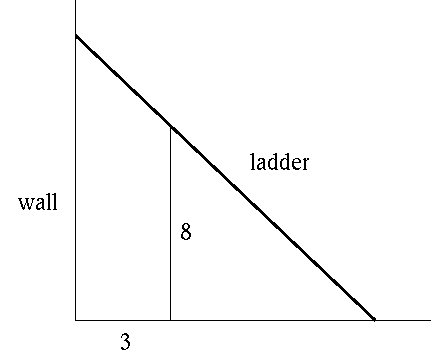
\includegraphics[width=0.5\textwidth]{MaxMin18A}
\end{enumerate}
\end{document}